\documentclass[journal abbreviation, manuscript]{copernicus}

\begin{document}

 %% \ SECTION 2
\section{The phydra package: structure \& features}

now explain in detail what the package is \& can do, what the structure is like

\subsection{Processes}
in xarray-simlab, (almost) everything is a process

\subsubsection{Components}
\subsubsection{Flows}
\subsubsection{Forcing & Physical Environment}

\subsection{Model development workflow}

%%% TWO-COLUMN FIGURES
%
%%f
\begin{figure*}[t]
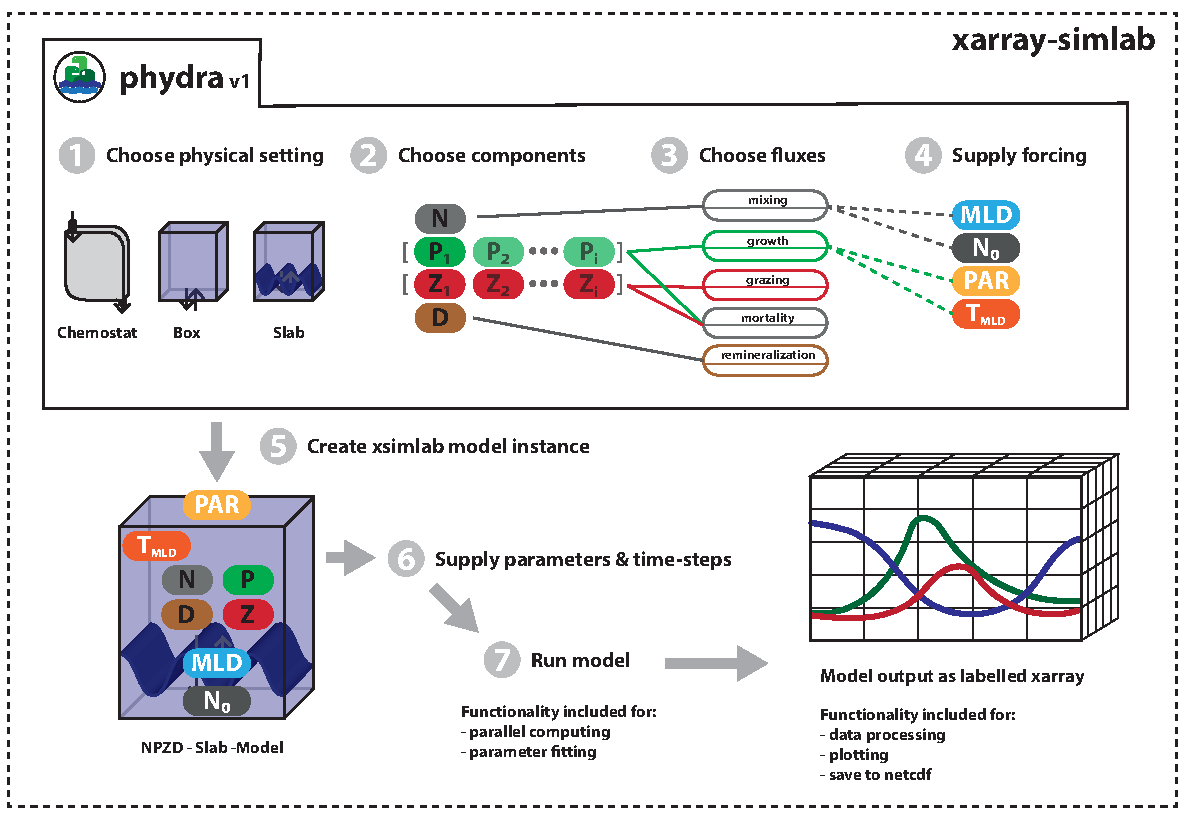
\includegraphics[width=12cm]{Figures/firstdraft_schematics/01__schematics_phydra.pdf}
\caption{TEXT}
\label{phydraschematics}
\end{figure*}

general explanation, and then go into detail below (see Figure \ref{phydraschematics})

% Everything below here is optional, it depends on what I can actually do in the package
\subsubsection{Dimensionality}
TEXT

\subsubsection{Runtime}
TEXT

\subsubsection{Model Diagnostics}
this is a relevant section, if Benoît can help me with creating the ODE visualization & model diagnostics.

\subsubsection{Parameter fitting}
this is a relevant section, if i manage to get some decent parameter fitting results for the example 1 and 3.. either only 3 or both, is my feeling. 

\end{document}